\chapter{Java 面向对象编程进阶 B}
\label{chp:Advanced-object-oriented-programming-2}

\section*{基本信息}
\sline
\begin{description}
\item[课程名称:] Java应用与开发
\item[授课教师:] 王晓东
\item[授课时间:] 第二周(根据校历,本周有两次课)
\item[参考教材:] 本课程参考教材及资料如下:
  \begin{itemize}
  \item 陈国君主编,Java程序设计基础(第5版),清华大学出版社,2015.5
  \item Bruce Eckel, Thinking in Java (3rd)
  \end{itemize}
\end{description}

\section*{教学目标}

\sline

\begin{enumerate}
\item 理解多态和虚方法调用的概念,掌握其用法
\item 掌握方法重载的方法
\item 掌握static属性、方法和初始化块的用法
\item 了解设计模式,掌握单例设计模式
\item 掌握final关键字的概念和使用方法
\end{enumerate}  

\section*{授课方式}

\sline
\begin{description}
\item[理论课:] 多媒体教学、程序演示
\item[实验课:] 上机编程
\end{description}

\newpage
\section*{教学内容}
\sline

%%%%%%%%%%%%%%%%%%%%%%%%%%%%%%%%%%%%%%%%%%%%%%%%%%%%%%%%%%%%%%
\section{多态性}

\subsection{多态的概念}

在Java中,子类的对象可以替代父类的对象使用称为{\hei 多态}。Java引用变量
与所引用对象间的类型匹配关系如下:

\begin{itemize}
\item 一个对象只能属于一种确定的数据类型,该类型自对象创建直至销毁不能
  改变。
\item 一个引用类型变量可能引用(指向)多种不同类型的对象——既可以引用其
  声明类型的对象,也可以引用其声明类型的子类的对象。
  \begin{javaCode}
    Person p = new Student(); //Student 是 Person 的子类  
  \end{javaCode}
\end{itemize}

\begin{figure}[htb]
  \centering
  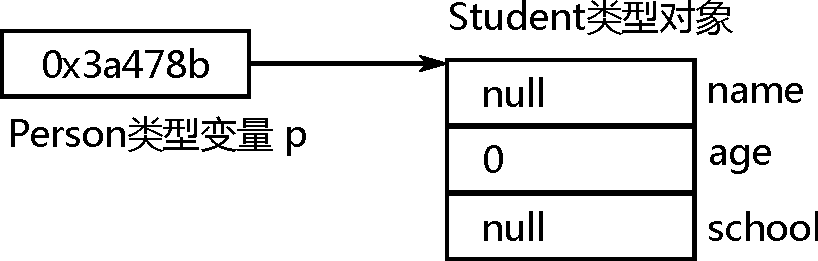
\includegraphics[width=0.6\textwidth]{images/Advanced-object-oriented-programming-2/fig-poly.pdf}
  \caption{Java多态}
  \label{fig:poly}
\end{figure}

多态性同样适用与引用类型数组元素。

\begin{javaCode}
  Person[] p = new Person[3]; 
  p[0] = new Student(); // 假设 Student 类继承了 Person 类
  p[1] = new Person();
  p[2] = new Graduate(); //假设 Graduate 类继承了 Student 类
\end{javaCode}

一个引用类型变量如果声明为父类的类型,但实际引用的是子类对象,该变量则不能再访问子类
中添加的属性和方法,这体现了父类引用对子类对象的能力屏蔽性。

\begin{javaCode}
  Student m = new Student();
  m.setSchool("ouc"); // 合法
  Person e = new Student();
  e.setSchool("ouc"); // 非法
\end{javaCode}

\subsection{多态用法示例}

\samp{Person.java}

\begin{javaCode}
  public class Person {...}
\end{javaCode}

\samp{Student.java}

\begin{javaCode}
  public class Student extends Person {
    private String school;

    public void setSchool(String school) {
      this.school = school;
    }

    public String getSchool() {
      return school;
    }

    @Override
    public String getInfo() {
      return super.getInfo() + "\tSchool: " + school;
    }
  }
\end{javaCode}

\samp{PolymorphismSample.java}

\begin{javaCode}
  public class PolymorphismSample {
    public void show(Person p) {
      System.out.println(p.getInfo());
    }
    
    public static void main(String[] args) {
      PolymorphismSample ps = new PolymorphismSample();
      Person p = new Person();
      ps.show(p);
      Student s = new Student();
      ps.show(s);
    }
  }
\end{javaCode}

\notice{多态提升方法通用性}

以上代码中,show()方法既可以处理Person类型的数据,又可以处理Student类型
的数据,乃至未来定义的任何Person子类类型的数据,即不必为相关的每种类型
单独声明一个处理方法,提高了代码的通用性。

\subsection{虚方法调用}

思考:一个引用类型的变量如果声明为父类的类型,但实际引用的是子类对象,
则该变量就不能再访问子类中添加的属性和方法。但如果此时调用的是父类中声
明过、且在子类中重写过的方法,情况如何?

补充代码。

\subsection{对象造型}

引用类型数据值之间的强制类型转换称为{\hei 造型(Casting)}。造型以下几种情况需要注意:

\begin{enumerate}
\item 从子类到父类的类型转换可以自动进行。
  \begin{javaCode}
    Person p = new Student();    
  \end{javaCode}
\item 在多态的情况下,有时我们可能需要恢复一个对象的本来面目,以发挥其
  全部潜力。从父类到子类的类型转换必须通过造型实现。
  \begin{javaCode}
    Person p1 = new Student();  
    Student s1 = (Student)p1;   // 合法
    Person p2 = new Person();   
    Student s2 = (Student)p2;  // 非法  
  \end{javaCode}
\item 无继承关系的引用类型间的转换是非法的。
  \begin{javaCode}
    String s = "Hello World!";
    Person p = (Person)s; // 非法  
  \end{javaCode}
\end{enumerate}

\subsection{instanceof运算符}

如果运算符instanceof左侧的变量当前时刻所引用的对象的{\hei\Red 真正类型}是
其右侧给出的类型{\Blue 或者是其子类},则整个表达式的结果为true。

\begin{javaCode}
class Person { --- }
class Student extends Person { --- }

public class Tool {
  public void distribute(Person p) {
    if (p instanceof Student) {
      System.out.println("处理 Student 类型及其子类类型对象");
    } else {
      System.out.println("处理 Person 类型及其子类类型对象");
    }
  }
}
\end{javaCode}

\begin{javaCode}
public class Test() {
  public static void main(String[] args) {
    Tool t = new Tool();
    Student s = new Student();
    t.distribute(t);
  }
}
\end{javaCode}

\subsection{虚方法调用和造型}

\codeset{package sample.oop.poly}

\begin{itemize}\small
\item VirtualMethodSample.java
\item Person.java
\item Student.java
\end{itemize}
  
强调以下与虚方法调用和造型相关的重点:
  
\begin{itemize}
\item 系统根据运行时对象的真正类型来确定具体调用哪一个方法,这一机制被称为
  {\hei\Blue 虚方法调用}。
\item 造型是引用类型数据值之间的强制类型转换。
\item instanceof运算符判断的是当前所引用对象的真正类型是什么,而不是声明的引用类型。
\end{itemize}

\section{方法重载}

\subsection{方法重载的概念}

在一个类中存在多个同名方法的情况称为{\hei 方法重载(Overload)}。Java对方法重载有以下要求:

\begin{itemize}
\item 重载方法参数列表必须不同。
\item 重载既可以用于普通方法,也可以用于构造方法。
\end{itemize}

\codeset{sample.oop.MethodOverloadSample.java}


\subsection{调用重载的构造方法}
  
\subsubsection{使用this调用当前类中重载构造方法}

可以在构造方法的第一行使用关键字this调用其它(重载的)构造方法。

\begin{javaCode}
  public class Person {
    ...
    public Person(String name,int age) {
      this.name = name;
      this.age = age;
    }
    public Person(String name) {
      this(name, 18);
    }
    ...
  }
\end{javaCode}

\notice{注意}

关键字this的此种用法只能用在构造方法中,且this()语句如果出
现必须位于方法体中代码的第一行。

\subsubsection{使用super调用父类构造方法}

\samp{Person.java}

\begin{javaCode}
  public class Person {
    ... (此处没有无参构造方法)
    public Person(String name, int age) {
      this.name = name;
      this.age = age;
    }
    ...
  }  
\end{javaCode}

\samp{Student.java}

\begin{javaCode}
  public class Student extends Person {
    private String school;
    public Student(String name, int age, String school) {
      super(name, age); // 显式调用父类有参构造方法
      this.school = school;
    }
    public Student(String school) { //编译出错
      // super(); // 隐式调用父类有参构造方法,则自动调用父类无参构造方法
      this.school = school;
    }
  }
\end{javaCode}

\notice{上述代码为什么会编译出错?}

{\Blue\hei 在Java类的构造方法中一定直接或间接地调用了其父类的构造方法(Object类除外)。}

\begin{enumerate}
\item 在子类的构造方法中可使用super语句调用父类的构造方法,其格式为super(<实参列表>)。
\item 如果子类的构造方法中既没有显式地调用父类构造方法,也没有使用this关键字调用同一个类
  的其他重载构造方法,则系统会默认调用父类无参数的构造方法,其格式为super()。
\item 如果子类构造方法中既未显式调用父类构造方法,而父类中又没有无参的构造方法,则编译出
  错。
\end{enumerate}

\codeset{sample.oop.ConstructorOverloadSample.java}
  


\subsection{对象构造/初始化细节}

\begin{description}
\item [第一阶段] 为新建对象的实例变量分配存储空间并进行默认初始化。
\item [第二阶段] 按下述步骤继续初始化实例变量:
  \begin{enumerate}
  \item 绑定构造方法参数;
  \item 如有this()调用,则调用相应的重载构造方法然后跳转到步骤5;
  \item 显式或隐式追溯调用父类的构造方法(Object类除外);
  \item 进行实例变量的显式初始化操作;
  \item 执行当前构造方法的方法体中其余的语句。 
  \end{enumerate}
\end{description}

\section{关键字static}

在Java类中声明{\hei\Red 属性、方法和内部类}时,可使用关键字static作为修饰符。

\begin{itemize}
\item static标记的属性或方法由整个类(所有实例)共享,如访问控制权限
  允许,可不必创建该类对象而直接用类名加“.”调用。
\item static成员也称{\hei\Blue “类成员”或“静态成员”},如“类属
  性”、“类变量”、“类方法”和“静态方法”等。
\end{itemize}

\subsection{static属性和方法}

\subsubsection{static属性}

\begin{itemize}
\item static属性由其所在类(包括该类所有的实例)共享。
\item 非static属性则必须依赖具体/特定的对象(实例)而存在。
\end{itemize}

\subsubsection{static方法}

要在static方法中调用其所在类的非static成员,应首先创建一个该类的对象,
通过该对象来访问其非static成员。

\codeset{sample.oop.StaticMemberAndMethodSample.java}


\subsection{初始化块}

\subsubsection{static初始化块}

在类的定义体中,方法的外部可包含static语句块,{\Red static块仅在其所属
  的类被载入时执行一次},通常用于初始化化static(类)属性。

\subsubsection{非static初始化块}

非static的初始化块在创建对象时被自动调用。

\codeset{sample.oop.StaticInitBlockSample.java}

\subsection{静态导入}

静态导入用于在一个类中导入其他类或接口中的static成员,语法格式如下:

\begin{javaCode}
  import static <包路径>.<类名>.*

  import static <包路径>.<类名>.<静态成员名>
\end{javaCode}

\samp{静态导入应用示例}

\begin{javaCode}
import static java.lang.Math.*;
public class Test {
  public static void main(String[] args) {
    double d = sin(PI * 0.45);
    System.out.println(d);
  }
}
\end{javaCode}

\subsection{Singleton设计模式}

所谓“模式”就是被验证为有效的常规问题的典型解决方案。{\hei 设计模式
  (Design Pattern)}在面向对象分析设计和软件开发中占有重要地位。好的设
计模式可以使我们更加方便的重用已有的成功设计和体系结构,极大的提高代码
的重用性和可维护性。

经典设计模式分类主要分为以下三大类:

\begin{description}
\item[创建型模式] 涉及对象的实例化,特点是不让用户代码依赖于对象的创建或排列方式,避免用户直接使用new创建对象。\\
  {\Red\kai 工厂方法模式、抽象工厂方法模式、生成器模式、原型模式和单例
    模式}
\item[行为型模式] 涉及怎样合理的设计对象之间的交互通信,以及合理为对象分配职责,让设计富有弹性、易维护、易复用。\\
  {\Blue\kai 责任链模式、命令模式、解释器模式、迭代器模式、中介者模式、
    备忘录模式、观察者模式、状态模式、策略模式、模板方法模式和访问者模
    式}
\item[结构型模式] 涉及如何组合类和对象以形成更大的结构,和类有关的结构型模式涉及如何合理使用继承机制,和对象有关的结构型模式涉及如何合理的使用对象组合机制。\\
  {\Mage\kai 适配器模式、组合模式、代理模式、享元模式、外观模式、桥接模
    式和装饰模式}
\end{description}


Singleton设计模式也称“单子模式”或“单例模式”。

\notice{采用调试方式讲解示例代码}

Singleton代码的特点包括以下几个方面:

\begin{enumerate}
\item 使用静态属性onlyone来引用一个“全局性”的Single实例。
\item 将构造方法设置为private的,这样在外界将不能再使用new关键字来创建该类的新实例。
\item 提供public static的方法getSingle()以使外界能够获取该类的实例,达到全局可见的效果。
\end{enumerate}

在任何使用到Single类的Java程序中(这里指的是一次运行中),需要确保只有
一个Single类的实例存在(如Web应用ServletContext全局上下文对象),则使用
该模式。

\section{关键字final}

在声明Java类、变量和方法时可以使用关键字final来修饰,以使其具有“终态”的特性:

\begin{enumerate}\kai
\item final标记的类不能被继承;
\item final标记的方法不能被子类重写;
\item final标记的变量(成员变量或局部变量)即成为常量,只能赋值一次;
\item final标记的成员变量必须在声明的同时或在每个构造方法中显式赋值,然后才能使用;
\item final不允许用于修饰构造方法、抽象类以及抽象方法。
\end{enumerate}

关键字final应用举例如下:

\begin{javaCode}
public final class Test {
  public static int totalNumber = 5;
  public final int id;
  public Test() {
    id = ++totalNumber; // 赋值一次
  }
  public static void main(String[] args) {
    Test t = new Test();
    System.out.println(t.id);
    final int i = 10;
    final int j;
    j = 20;
    j = 30;  // 非法
  }
}
\end{javaCode}

\section{课后习题}

\tta{简答题}
\begin{enumerate}
\item 为什么建议Java类需要编写无参构造方法,哪怕该方法什么都没做?
\item 关键字static都可以用来修饰Java类的那些成员?
\end{enumerate}

\tta{小编程}
\begin{enumerate}
\item 练习本节中所有示例代码,理解并掌握其用法。
\item 自行调试单例设计模式程序,学习Eclipse的Debug方法,练习断点、单
  步执行、跟进方法等操作,查看内存变化。
\end{enumerate}